% ieee-twocolumn-sample.tex -- IEEE journal / Transactions baseline sample
%
% Provenance: written for this repository on 2026-11-18. The upstream
% latex-document-skill project ships only PNG previews under examples/ and
% has never included a .tex sample (see references/UPSTREAM.md and
% ASSET-GAP.md). The preview PNGs beside this file (ieee-twocolumn.png,
% ieee-twocolumn-p1.png, ieee-twocolumn-p2.png) come from the pinned fork
% snapshot and illustrate the expected two-column layout.
%
% Demonstrates (per SKILL.md): \documentclass[journal,10pt]{IEEEtran} with
% abstract, index terms (keywords), one single-column figure, one
% single-column table, one full-width table* float, and a numeric
% thebibliography. Layout rules follow
% references/ieee-journal-twocolumn-guide.md: no geometry overrides,
% [!t] float placement, \columnwidth for single-column figures vs.
% \textwidth inside table*, and hidelinks hyperref.
%
% Compile (2-3 passes for stable references):
%   pdflatex ieee-twocolumn-sample.tex
% Switch to xelatex (+fontspec) if you add non-ASCII glyphs to body text.

\documentclass[journal,10pt]{IEEEtran}

\usepackage{cite}
\usepackage{amsmath,amssymb,amsfonts}
\usepackage{graphicx}
\usepackage{textcomp}
\usepackage{xcolor}
\usepackage{array}
\usepackage{booktabs}
\usepackage{tikz}
\usetikzlibrary{positioning}
\usepackage[hidelinks]{hyperref}

\begin{document}

\title{An Efficient Baseline for IEEE Two-Column Manuscripts\\
{\footnotesize A compilable sample for the latex-document skill}}

\author{J.~A.~Doe,~\IEEEmembership{Member,~IEEE},%
        R.~R.~Roe,~\IEEEmembership{Student~Member,~IEEE},%
        and~M.~M.~Moe,~\IEEEmembership{Senior~Member,~IEEE}%
\thanks{Manuscript received November 18, 2026; revised November 18, 2026.
This work was supported by the Example Institution under Grant~X000000.}%
\thanks{J.~A.~Doe is with the Department of Example Systems, University of
Exampleville, Exampleville, EX1 2AB, Country (e-mail: j.doe@example.org).}%
\thanks{R.~R.~Roe and M.~M.~Moe are with the Example Research Laboratory,
Exampleville, EX3 4CD, Country (e-mail: \{r.roe, m.moe\}@example.org).}}

\markboth{IEEE Transactions on Example Systems, Vol.~XX, No.~X, 2026}%
{Doe \MakeLowercase{\textit{et al.}}: An Efficient Baseline for IEEE Two-Column Manuscripts}

\maketitle

\begin{abstract}
This document is a self-contained baseline for IEEE Transactions-style
two-column manuscripts. It exercises the elements called out in the skill
description: a journal-class preamble, an abstract, index terms, a
single-column figure, a single-column table, a full-width table* float, and
a numeric bibliography. Copy this file, replace the placeholder content,
and keep the layout rules from the IEEE two-column guide: trust the class
geometry, place floats with [!t], size single-column figures with
\textbackslash columnwidth, and reserve star floats for content that
genuinely overflows one column.
\end{abstract}

\begin{IEEEkeywords}
IEEEtran, two-column layout, camera-ready, LaTeX, typography.
\end{IEEEkeywords}

\section{Introduction}
\IEEEPARstart{T}{his} sample uses the standard journal opening: a drop-cap
first paragraph produced by \textbackslash IEEEPARstart, followed by the
motivation, the contribution list, and the paper organization. The running
header on page~2 onward comes from \textbackslash markboth in the preamble
block above.

The contributions of this sample are threefold:
\begin{enumerate}
  \item a minimal, compilable IEEEtran journal baseline;
  \item float examples that follow the two-column rules
        (Fig.~\ref{fig:overview}, Tables~\ref{tab:single} and~\ref{tab:full});
  \item a numeric reference list in IEEE style.
\end{enumerate}

\section{Method}
The toy objective optimized by this sample framework is
\begin{equation}
  \mathcal{L}_{\text{total}} = \mathcal{L}_{\text{task}}
  + \lambda\,\mathcal{L}_{\text{reg}},
  \label{eq:loss}
\end{equation}
where $\mathcal{L}_{\text{task}}$ is the task loss,
$\mathcal{L}_{\text{reg}}$ is a regularization term, and $\lambda$ balances
the two. Prior work~\cite{doe2024,roe2023} established the two-column
pipeline; the LaTeX tooling background is covered
in~\cite{mittelbach2004,carlisle2019}.

\begin{figure}[!t]
  \centering
  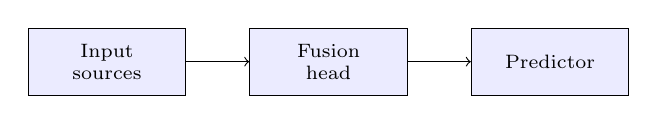
\begin{tikzpicture}[every node/.style={font=\scriptsize},
                      box/.style={draw, fill=blue!8, minimum width=2.0cm,
                                  minimum height=0.85cm, align=center}]
    \node[box] (src)  {Input\\sources};
    \node[box, right=0.8cm of src] (fuse) {Fusion\\head};
    \node[box, right=0.8cm of fuse] (out) {Predictor};
    \draw[->] (src)  -- (fuse);
    \draw[->] (fuse) -- (out);
  \end{tikzpicture}
  \caption{Single-column figure: a three-stage pipeline drawn at column
  width. Caption text only -- IEEEtran prepends ``Fig.~N.'' automatically.}
  \label{fig:overview}
\end{figure}

\section{Experiments}
Fig.~\ref{fig:overview} shows the pipeline. Table~\ref{tab:single} is a
single-column table that fits one column with \textbackslash scriptsize
type and tightened column separation. Table~\ref{tab:full} is the
full-width counterpart (table*) used only because seven columns do not fit
a single column.

\begin{table}[!t]
  \renewcommand{\arraystretch}{1.1}
  \setlength{\tabcolsep}{2pt}
  \caption{Single-Column Comparison on the Example Benchmark}
  \label{tab:single}
  \centering
  \scriptsize
  \begin{tabular}{@{}lrr@{}}
    \toprule
    Method & Metric A & Metric B \\
    \midrule
    Baseline       & 0.643 & 0.589 \\
    Re-implemented & 0.701 & 0.612 \\
    Ours           & \textbf{0.812} & \textbf{0.745} \\
    \bottomrule
  \end{tabular}
\end{table}

\begin{table*}[!t]
  \renewcommand{\arraystretch}{1.15}
  \setlength{\tabcolsep}{5pt}
  \caption{Full-Width Comparison Across Example Datasets (Spans Both Columns)}
  \label{tab:full}
  \centering
  \footnotesize
  \begin{tabular}{@{}lcccccc@{}}
    \toprule
    Dataset & Model & Params (M) & FLOPs (G) & Top-1 (\%) & Latency (ms) & Memory (MB) \\
    \midrule
    Example-A & Baseline & 21.3 & 4.1 & 74.9 & 12.8 & 512 \\
    Example-A & Ours     & 19.7 & 3.6 & \textbf{78.2} & 11.4 & 498 \\
    Example-B & Baseline & 21.3 & 4.1 & 71.5 & 12.9 & 517 \\
    Example-B & Ours     & 19.7 & 3.6 & \textbf{75.1} & 11.5 & 501 \\
    \bottomrule
  \end{tabular}
\end{table*}

\section{Conclusion}
This baseline compiles with pdfLaTeX in two to three passes and can be
extended with real content. For Greek letters, em-dashes, or non-ASCII
author names in body text, switch to xelatex with fontspec as described in
the IEEE two-column guide, and re-run the self-check before submission.

\begin{thebibliography}{10}

\bibitem{doe2024}
J.~A.~Doe and M.~M.~Moe, ``A baseline for two-column manuscripts,''
\emph{IEEE Trans. Example Syst.}, vol.~10, no.~2, pp.~100--110, Jun.~2024,
doi: 10.1109/EXAMPLE.2024.123456.

\bibitem{roe2023}
R.~R.~Roe, ``Early results on column-aware float placement,'' in
\emph{Proc. IEEE Example Conf.}, Exampleville, Country, 2023, pp.~1--8.

\bibitem{mittelbach2004}
F.~Mittelbach and M.~Goossens, \emph{The \LaTeX\ Companion}, 2nd~ed.
Boston, MA, USA: Addison-Wesley, 2004.

\bibitem{carlisle2019}
D.~Carlisle, ``booktabs -- Publication quality tables,'' CTAN, 2019.
[Online]. Available: https://ctan.org/pkg/booktabs

\bibitem{ieee2026}
IEEE, ``IEEE editorial style manual for authors,'' IEEE, Piscataway, NJ,
USA, Tech. Rep., 2026.

\end{thebibliography}

\end{document}
